\documentclass[12pt]{article}
\usepackage[left=2cm, top=2cm, right=2cm, bottom=2cm]{geometry}
\usepackage[utf8]{inputenc}      % accents dans le source
\usepackage[T1]{fontenc}
\usepackage[french]{babel}
\usepackage{graphicx}
\usepackage{graphics}
\usepackage{amsmath}
\usepackage{tikz}
\usepackage{xcolor} 
\usepackage{mathtools}
\usepackage{parskip}
\usepackage{subcaption}
\usepackage[export]{adjustbox}

\title{\vspace{-2cm}\textbf{TP 2 - Ondes progressives ultrasonores}}
\author{MENARD Alexandre - VIEILLEDENT Florent}
% \setlength{\parindent}{1cm}
\date{\vspace{-0.5cm}}

\begin{document}
\maketitle

L'acoustique est l'étude des ondes sonores dans différents milieux. Elle trouve des applications dans le développement des chambres
anéchoïques où l'on cherche à minimiser au maximum les perturbations sonores pour permettre des mesures précises sur le son émis par des appareils par exemple. 
Notre travail ici consistera à caractériser les ondes sonores progressives ultrasonores par observation qualitative. Nous proposerons
deux protocoles pour déterminer la célérité de ces dernières et nous mesurerons les coefficients de transmission et réflexion pour différents matériaux.

\section{Mesure de la célérité du son}
\subsection{Modèle}
En suppose que l'onde émise est parfaitement sinusoïdale et que la dissipation de l'énergie de l'onde sur la distance est négligeable, l'amplitude $A$ restant donc constante. 
Nous pouvons modéliser la propagation de cette dernière avec $k=\frac{2\pi}{\lambda}$, $\omega$ la pulsation et $\phi$ la phase à l'origine:
\begin{align}
	y(x, t) = A \sin(\omega t - kx + \phi)
\end{align}

Si deux signaux (émis ou reçus) sont en phase, on a alors en deux positions $x_1$ et $x_2$:
\begin{align*}
	y(x_1, t) = y(x_2, t) & \Rightarrow |x_1 - x_2| = n\lambda
\end{align*}

\subsection{Génération et caractérisation d'une onde sonore}
L'émetteur sonore est composé d'un matériau dit piézo-électrique capable de se déformer sous un champ électrique. Ainsi, soumis à un champ électrique
le matériau va se déformer et générer un déplacement du milieu donc une onde sonore. Pour une première approche, nous suivons le protocole
expérimental dans la section \textbf{1.1}. Nous observons alors des signaux ayant [\dots]


\subsection{Protocole expérimental}
Nous suivrons les protocoles expérimentaux 1 et 2 fournis dans la section \textbf{1.2}. Nous utilisons le mode \textit{trigger}
de l'oscilloscope pour stabiliser la forme du signal en synchronisant le balayage horizontal à un certains point du signal et faciliter la lecture de ce dernier.
La fiche technique de l'émetteur précise une fréquence émise \textbf{autour} de 40kHz, on prend donc $\nu = 40 \pm 0.2 \text{kHz}$ pour tenir compte de l'absence d'une incertitude précise. 
Les positions des récépteurs et de l'émetteur sont notés $x_{re_1}, x_{re_2}, x_{em}$ et ont des incertitudes associées
$\delta x = 0.1cm$ que l'on détermine par les graduations fournies par le rail gradué. 
\begin{figure}[!htbp]
	\centering
	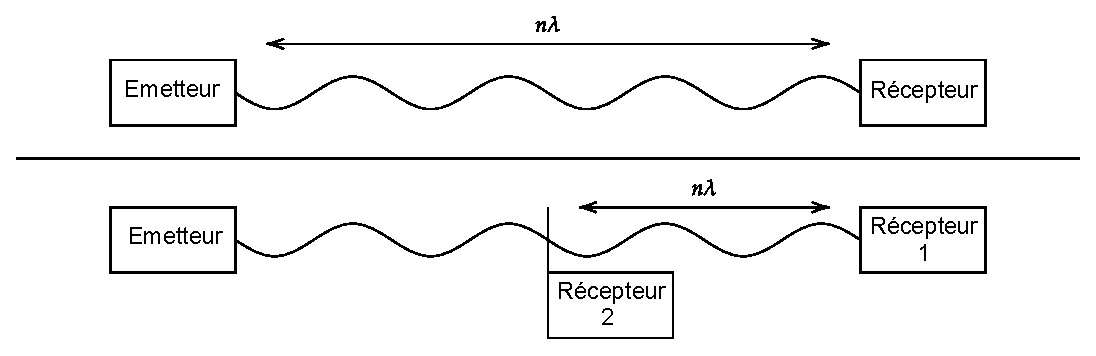
\includegraphics[width=0.6\textwidth]{img/schema}
	\hfill
	\caption{Schéma des deux protocoles 1 et 2}
\end{figure}
\section{Mesure des coefficients de transmission et réflexion}


\break
\section*{Annexes}
\subsection*{Table de données pour la }
\end{document}